\documentclass[12pt,titlepage]{article}
\usepackage[margin=1.25in]{geometry}
\usepackage{graphicx,amsmath,blindtext,minted}

%% Variables definition
\newcommand{\vSubject}{Advance Data Base}
\newcommand{\vSubtitle}{MySQL Basics and Data Definition Language}
\newcommand{\vName}{Muhammad Baihaqi Aulia Asy'ari}
\newcommand{\vNIM}{2241720145}
\newcommand{\vClass}{2I}
\newcommand{\vDepartment}{Information Technology}
\newcommand{\vStudyProgram}{D4 Informatics Engineering}

%% [START] Tikz related stuff
\usepackage{tikz}
\usetikzlibrary{svg.path,calc,shapes.geometric,shapes.misc}
\tikzstyle{terminator} = [rectangle, draw, text centered, rounded corners = 1em, minimum height=2em]
\tikzstyle{preparation} = [chamfered rectangle, chamfered rectangle sep=0.75em, draw, text centered, minimum height = 2em]
\tikzstyle{process} = [rectangle, draw, text centered, minimum height=2em]
\tikzstyle{decision} = [diamond, aspect=2, draw, text centered, minimum height=2em]
\tikzstyle{data}=[trapezium, draw, text centered, trapezium left angle=60, trapezium right angle=120, minimum height=2em]
\tikzstyle{connector} = [line width=0.25mm,->]
%% [END] Tikz related stuff

%% [START] Fancy header related stuff
\usepackage{fancyhdr}
\pagestyle{fancy}
\setlength{\headheight}{15pt} % compensate fancyhdr style
\fancyhead{}
\fancyfoot{}
\fancyfoot[L]{\thepage}
\fancyfoot[R]{\textit{\vSubject - \vSubtitle}}
\renewcommand{\footrulewidth}{0.4pt}% default is 0pt, overline for footer
%% [END] Fancy header related stuff

%% [START] Custom tabular command related stuff
\usepackage{tabularx}
\newcommand{\details}[2]{
    #1 & #2  \\
}
%% [END] Custom tabular command related stuff

%% [START] Figure related stuff
\newcommand{\image}[3][1]{
    \begin{figure}[h]
        \centering
        \includegraphics[#1]{#2}
        \caption{#3}
        \label{#3}
    \end{figure}
}
%% [END] Figure related stuff

%%
\usepackage{pgf-umlcd}

\renewcommand{\umldrawcolor}{black}
\renewcommand{\umlfillcolor}{white}
%%

%% [BEGIN] Custom enumerator
\usepackage{enumitem}
%% [END] Custom enumerator

%% [BEGIN] Paragraph indent
\usepackage{indentfirst}
%% [END] Paragraph indent

\begin{document}
\begin{titlepage}
    \centering
    \vfill
    {\bfseries\LARGE
        \vSubject\\
        \vskip0.25cm
        \vSubtitle
    }
    \vfill
    
\includegraphics[width=6cm]{images/polinema-logo.png}
    \vfill
    {
        \textbf{Name}\\
        \vName\\
        \vskip0.5cm
        \textbf{NIM}\\
        \vNIM\\
        \vskip0.5cm
        \textbf{Class}\\
        \vClass\\
        \vskip0.5cm
        \textbf{Department}\\
        \vDepartment\\
        \vskip0.5cm
        \textbf{Study Program}\\
        \vStudyProgram
    }
\end{titlepage}

\newpage

\section*{Practicum}

\begin{enumerate}
    \item Buka prompt jalankan perintah berikut ini :\\
    C:$\backslash>$Program Files$\backslash$xampp$\backslash$mysql$\backslash$bin$>$mysql -u root -p (enter)\\
    \includegraphics[width=0.9\textwidth]{images/figures/practicum-1.PNG}
    \item Buatlah sebuah database dengan nama db\textunderscore polinema\\
    \includegraphics[width=0.9\textwidth]{images/figures/practicum-2.PNG}
    \item Buatlah beberapa tabel dalam database tersebut sesuai dengan kriteria berikut: \\
    Tabel \texttt{prodi} \\
    \begin{tabular}{|p{0.2\textwidth}|p{0.6\textwidth}|}
        \hline
        \textbf{Field} & \textbf{Type Data} \\
        \hline
        kode\textunderscore prodi & VARCHAR (6) PRIMARY KEY \\
        \hline
        nama\textunderscore prodi & VARCHAR (30) \\
        \hline
    \end{tabular}
    \\
    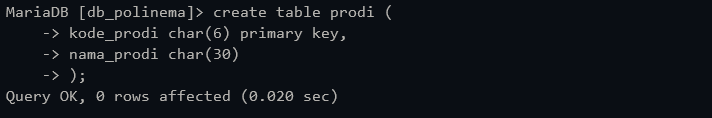
\includegraphics[width=0.8\textwidth]{images/figures/practicum-4.PNG}
    \newpage
    \item Tabel \texttt{mahasiswa} \\
    \begin{tabular}{|p{0.2\textwidth}|p{0.6\textwidth}|}
        \hline
        \textbf{Field} & \textbf{Type Data} \\
        \hline
        nim & INT (8) PRIMARY KEY \\
        \hline
        nama\textunderscore mhs & VARCHAR (50) \\
        \hline
        jenis\textunderscore kelamin & ENUM ('L','P') DEFAULT 'L' \\
        \hline
        alamat & VARCHAR (50) \\
        \hline
        kota & VARCHAR (20) DEFAULT 'MALANG' \\
        \hline
        asal\textunderscore sma & VARCHAR (30) \\
        \hline
        no\textunderscore hp & VARCHAR (12) \\
        \hline
        umur & INT \\
        \hline
        kode\textunderscore prodi & VARCHAR (6) FOREIGN KEY fk0 (kode\textunderscore prodi) REFERENSCES prodi (kode\textunderscore prodi) \\
        \hline
    \end{tabular}
    \\
    \includegraphics[width=0.8\textwidth]{images/figures/practicum-3.PNG}
    \item Tabel \texttt{mata\textunderscore kuliah} \\
    \begin{tabular}{|p{0.2\textwidth}|p{0.6\textwidth}|}
        \hline
        \textbf{Field} & \textbf{Type Data} \\
        \hline
        mk\textunderscore id & VARCHAR (10) PRIMARY KEY \\
        \hline
        nama\textunderscore mk & VARCHAR (50) \\
        \hline
        jumlah\textunderscore jam & FLOAT (4,2) \\
        \hline
        sks & INTEGER \\
        \hline
    \end{tabular}
    \\
    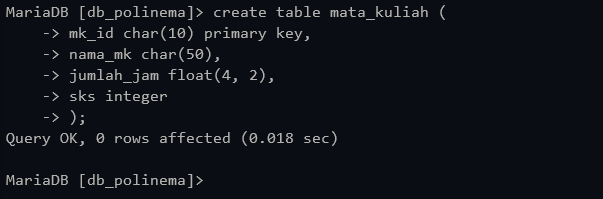
\includegraphics[width=0.8\textwidth]{images/figures/practicum-5.PNG}
    \newpage
    \item Tabel \texttt{ruang} \\
    \begin{tabular}{|p{0.2\textwidth}|p{0.6\textwidth}|}
        \hline
        \textbf{Field} & \textbf{Type Data} \\
        \hline
        ruang\textunderscore id & VARCHAR (10) PRIMARY KEY \\
        \hline
        nama\textunderscore ruang & VARCHAR (50) \\
        \hline
        kapasitas & INTEGER \\
        \hline
    \end{tabular}
    \\
    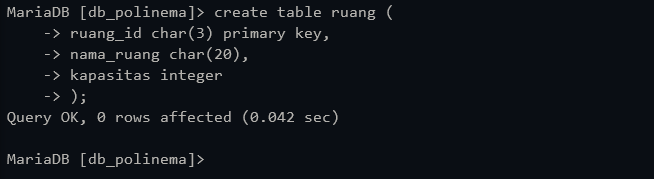
\includegraphics[width=0.8\textwidth]{images/figures/practicum-6.PNG}
    \item Tabel \texttt{dosen} \\
    \begin{tabular}{|p{0.2\textwidth}|p{0.6\textwidth}|}
        \hline
        \textbf{Field} & \textbf{Type Data} \\
        \hline
        nidn & INTEGER (20) PRIMARY KEY \\
        \hline
        nama\textunderscore dosen & VARCHAR (50) \\
        \hline
        status & ENUM ('PNS','KONTRAK') DEFAULT 'PNS' \\
        \hline
        jenis\textunderscore kelamin & ENUM ('L','P') DEFAULT 'L' \\
        \hline
        no\textunderscore hp & VARCHAR (15) \\
        \hline
    \end{tabular}
    \\
    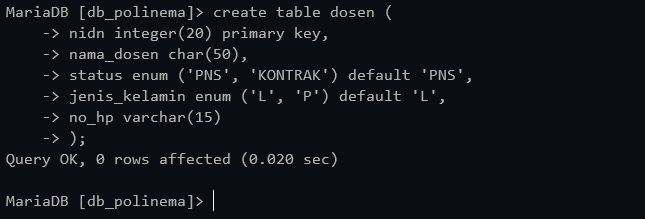
\includegraphics[width=0.8\textwidth]{images/figures/practicum-7.PNG}
    \newpage
    \item \textbf{$<$Soal$>$} \\ Tambahkan sebuah kolom agama (varchar(10)) pada tabel mahasiswa sebagai kolom terakhir \\
    \textcolor{red}{Catat : Buat Screenshot dari perintah yang anda ketikkan} \\
    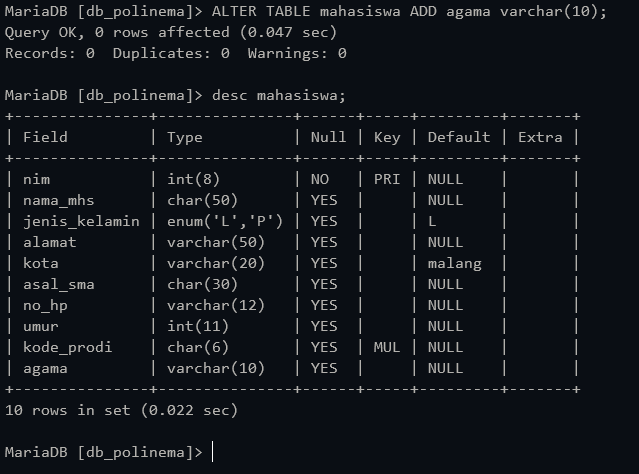
\includegraphics[width=0.8\textwidth]{images/figures/practicum-8.PNG}
    \item \textbf{$<$Soal$>$} \\ Tambahkan kolom alamat(varchar(50)) pada tabel dosen sebagai kolom terakhir \\
    \textcolor{red}{Catat : Buat Screenshot dari perintah yang anda ketikkan} \\
    \includegraphics[width=0.8\textwidth]{images/figures/practicum-9.PNG}
    \newpage
    \item \textbf{$<$Soal$>$} \\ Lakukan insert data ke dalam tabel-tabel yang ada pada pada database \newline db\textunderscore polinema sesuai dengan field, tipe data dan panjang datanya \\
    \textcolor{red}{Catat : Buat Screenshot dari perintah yang anda ketikkan} \\
    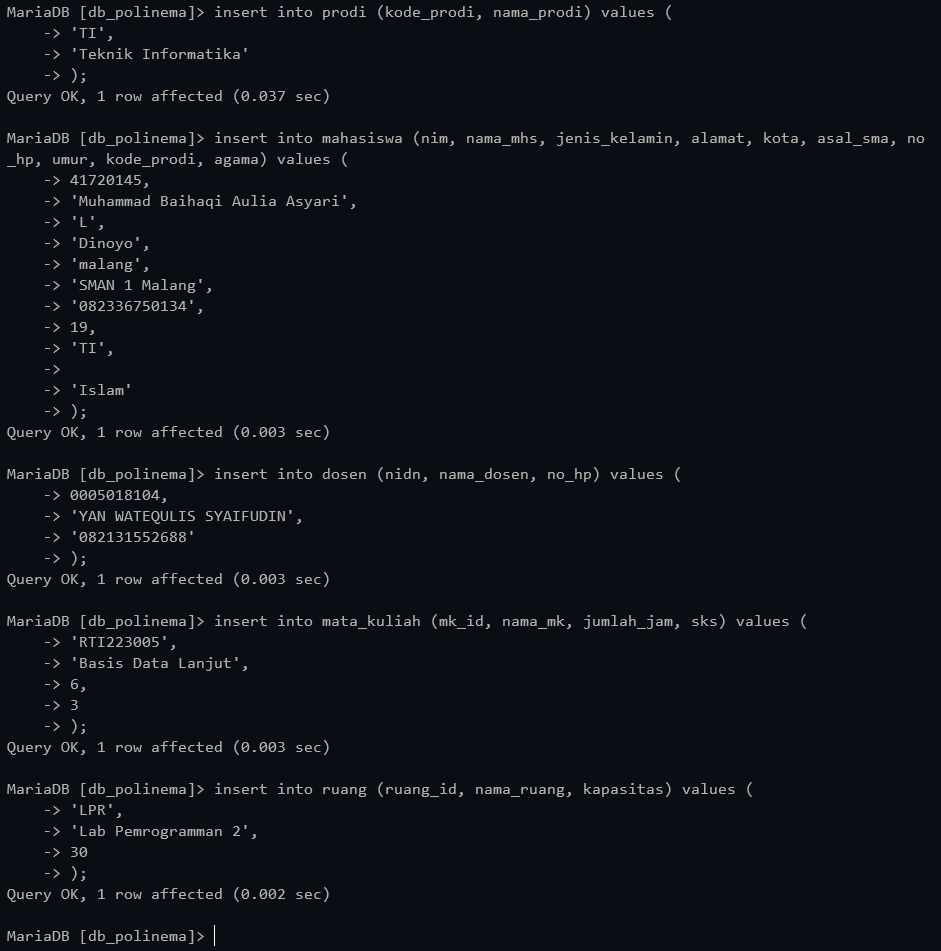
\includegraphics[width=0.8\textwidth]{images/figures/practicum-10.PNG}
    \item \textbf{$<$Soal$>$} \\ Tampilkan semua tabel yang ada didalam database db\textunderscore polinema \\
    \textcolor{red}{Catat : Buat Screenshot dari perintah yang anda ketikkan} \\
    \includegraphics[width=0.8\textwidth]{images/figures/practicum-11.PNG}\newpage
    \item \textbf{$<$Soal$>$} \\ Tampilkan semua isi tabel yang ada didalam tabel mahasiswa \\ 
    \textcolor{red}{Catat : Buat Screenshot dari perintah yang anda ketikkan} \\
    \includegraphics[width=0.8\textwidth]{images/figures/practicum-12.PNG}
    \item \textbf{$<$Soal$>$} \\ Tampilkan struktur(metadata) tabel mahasiswa 
    \textcolor{red}{Catat : Buat Screenshot dari perintah yang anda ketikkan} \\
    \includegraphics[width=0.8\textwidth]{images/figures/practicum-13.PNG}
    \newpage
    \item \textbf{$<$Soal$>$} \\ hilangkan kolom asal\textunderscore sma yang terdapat didalam tabel mahasiswa \\ 
    \textcolor{red}{Catat : Buat Screenshot dari perintah yang anda ketikkan} \\
    \includegraphics[width=0.8\textwidth]{images/figures/practicum-14.PNG}
\end{enumerate}

\newpage
\section*{Tugas}
\begin{enumerate}
    \item \textbf{Buatlah basis data Akademik dengan data sebagai berikut :} \\
    \begin{tabular}{|l|l|l|l|l|l|l|l|}
        \hline
        No\textunderscore Mhs & Nama\textunderscore mhs & Jurusan & Kd\textunderscore MK & Nama\textunderscore mk & Kd\textunderscore Dosen & Nm\textunderscore Dosen & nilai \\
        \hline
        1921001 & Aminah & MI & MI350 & Basis Data & B104 & Ati & 85 \\
        \hline
        1921001 & Budiman & MI & MI465 & Pemrograman & B105 & Dita & 87 \\
        \hline
        1921002 & Carina & MI & MI465 & Pemrograman & B105 & Dita & 85 \\
        \hline
        1921003 & Della & TI & TI201 & Mobile & C102 & Leo & 78 \\
        \hline
        1921004 & Firda & TI & TI201 & Mobile & C102 & Leo & 80 \\
        \hline
    \end{tabular}
    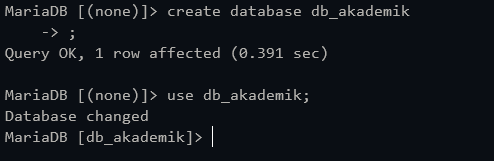
\includegraphics[width=0.8\textwidth]{images/figures/tugas-1_preamble.PNG}
    \begin{enumerate}
        \item deskripsikan struktur data dari table-tabel berikut serta isikan datanya: \\
        Tabel Mahasiswa \{No\textunderscore Mhs, Nama\textunderscore mhs\} \\
        Tabel Mata\textunderscore Kuliah \{Kd\textunderscore MK, Nama\textunderscore MK\} \\
        Tabel nilai \{No\textunderscore Mhs, Kode\textunderscore MK\} \\
        tambahkan kolom Jurusan pada tabel Mahasiswa di kolom terakhir \\
        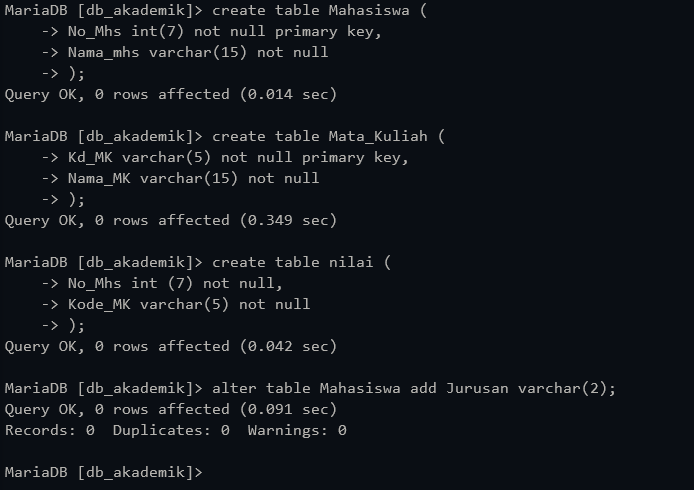
\includegraphics[width=0.8\textwidth]{images/figures/tugas-1_a_1.PNG}
        \\
        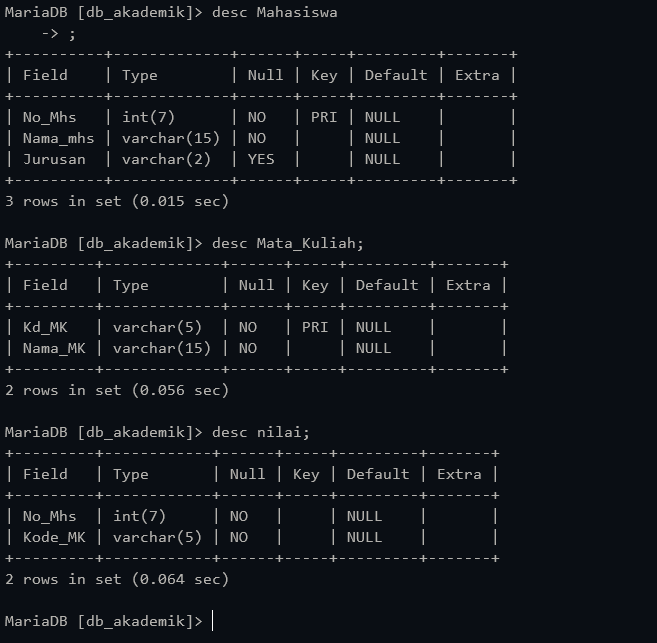
\includegraphics[width=0.8\textwidth]{images/figures/tugas-1_a_2.PNG}
        \item tambahkan kolom Kode Dosen pada tabel Mata\textunderscore Kuliah
        \item tambahkan kolom nilai pada tabel nilai serta berikanlah kunci foreign key
        \item tambahkan Tabel Dosen dengan atributnya Kd\textunderscore Dosen dan Nama Dosen
        \item tampilkan semua data yang ada pada tiap tabel
    \end{enumerate}
    \item \textbf{Buatlah basis data Pegawai yang terdiri dari tabel sebagai berikut :}
    \begin{tabular}{|l|l|l|l|l|l|}
        \hline
        Noproyek & NamaProyek & Nopegawai & NamaPegawai & Golongan & BesarGaji \\
        \hline
        NP001 & BRR & Peg01 & Anton & A & 1.000.000 \\
        \hline
        NP001 & BRR & Peg02 & Paula & B & 900.000 \\
        \hline
        NP001 & BRR & Peg06 & Koko & C & 750.000 \\
        \hline
        NP002 & PEMDA & Peg01 & Anton & A & 1.000.000 \\
        \hline
        NP002 & PEMDA & Peg12 & Sita & B & 900.000 \\
        \hline
        NP002 & PEMDA & Peg14 & Yusni & B & 900.000 \\
        \hline
        NP003 & CBR & Peg02 & Paula & B & 900.000 \\
        \hline
        NP003 & CBR & Peg03 & Daniar & C & 750.000 \\
        \hline
        NP003 & CBR & Peg04 & Lubis & C & 750.000 \\
        \hline
        NP004 & ASK & Peg07 & Keni & B & 900.000 \\
        \hline
        NP004 & ASK & Peg08 & Sofi & B & 900.000 \\
        \hline
        NP004 & ASK & Peg06 & Yuni & C & 750.000 \\
        \hline
        NP005 & OB & Peg15 & Udin & D & 500.000 \\
        \hline
        NP005 & OB & Peg16 & Didit & D & 500.000 \\
        \hline
        NP005 & OB & Peg17 & Dani & D & 500.000 \\
        \hline
    \end{tabular}
    \begin{enumerate}
        \item Deskripsikan struktur data dari table-tabel berikut serta isikan datanya: \\
        Table Pegawai \{Nopegawai, NamaPegawai\} \\
        Tabel Golongan \{Golongan\} \\
        Tabel Proyek \{Noproyek\} \\
        Tabel Proyekpegawai \{Noproyek\} \\
        \item Tambahkan kolom Golongan pada tabel Pegawai di kolom terakhir
        \item Tambahkan kolom BesarGaji pada tabel Golongan di kolom terakhir
        \item Tambahkan kolom NamaProyek pada table Proyek
        \item Tambahkan kolom NoPegawai pada table Proyekpegawai serta berikanlah kunci foreign key
        \item Tampilkan semua data yang ada pada tiap tabel
    \end{enumerate}
\end{enumerate}

\end{document}